\section{Regionale Datenarchitektur zur Abdeckung der Data Science Use Cases}
\label{sec:regionale-architektur}

Als erstes wird die Datenarchitektur vorgestellt, 
die für die KFZ Betrugserkennung und die KV-Kündiger Prognose
benötigt wird. 
Sie müsste mehrfach in gleicher Form aufgebaut werden.
Je einmal pro Region,
für die diese Anwendungsfälle gesammelt betrachtet werden.
Dabei dürfen die Regionen sich nicht über die Grenzen 
eines Datenraums hinaus erstrecken, 
in dem die schützenswerten Daten verarbeite weren müssen.
Wie genau die Regionen dann geschnitten werden,
ist eine Entscheidung der Allianz SE.
Denkbar wären verschiedene Skalierungen, 
wie z.B. Deutschland, DACH Raum oder EU-weit. 

Diese regional aufzubauende Datenarchitektur ist in 
Abb. \ref{fig:datenarchitektur-regional} dargestellt.
Im Kern der Architektur befinden sich ein Data Lake
und ein Data Warehouse.
Hier werden die Daten aus den relevanten Datenquellen persistiert.
Bei der Allianz SE gibt es viele strukturierte Datenquellen,
darunter Kundendaten, Vertragsdaten, historische Schadensdaten und Betrugsfälle, 
Leistungsabrechnungen, Fahrzeugtelemetriedaten, etc.
Dazu kommen sozioökonomische Daten je Postleitzahl, 
welche aus externen Erhebungen entnommen werden.
Diese strukturierten Daten werden in automatisierter
Batchverarbeitung jede Nacht 
(in Abb. \ref{fig:datenarchitektur-regional} dargestellt als ''aktuell'')
in das Data Warehouse übertragen.

\begin{figure}[tbh]
    \centering 
    %\vspace{0.5cm}
    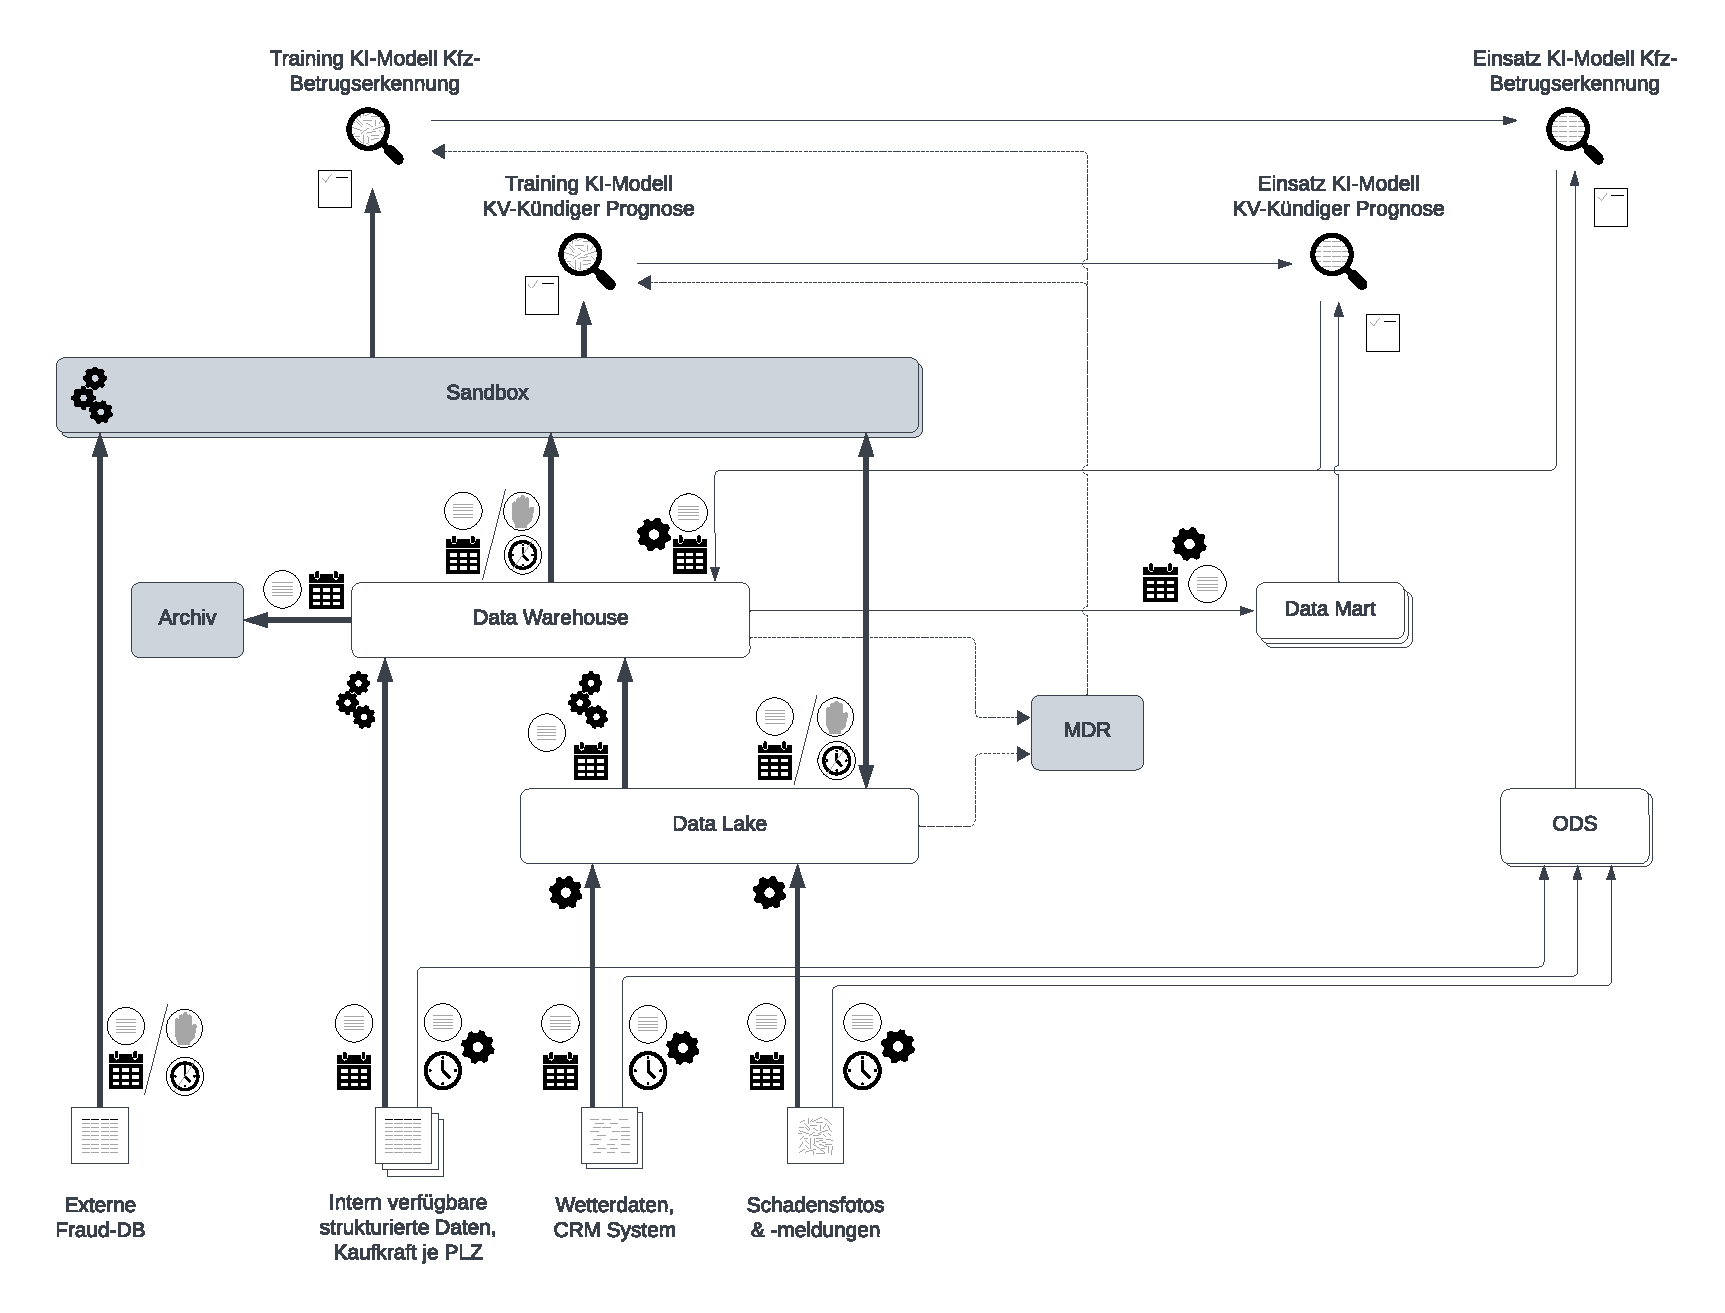
\includegraphics[width=\textwidth]{images/Diagram_regionale_Datenarchitektur.pdf}
    \caption{Detaillierte regionale Datenarchitektur}\label{fig:datenarchitektur-regional}
\end{figure}

